% Created 2020-01-13 Mon 10:48
\documentclass[11pt]{article}
\usepackage[utf8]{inputenc}
\usepackage[T1]{fontenc}
\usepackage{fixltx2e}
\usepackage{graphicx}
\usepackage{longtable}
\usepackage{float}
\usepackage{wrapfig}
\usepackage{rotating}
\usepackage[normalem]{ulem}
\usepackage{amsmath}
\usepackage{textcomp}
\usepackage{marvosym}
\usepackage{wasysym}
\usepackage{amssymb}
\usepackage{hyperref}
\tolerance=1000
\usepackage{minted}
\usepackage{amsthm}
\usepackage[margin=1.0in]{geometry}
\setlength{\parindent}{0pt}
\setlength{\parskip}{\baselineskip}
\author{Thomas Alford}
\date{\today}
\title{Ph21 Problem Set 1}
\hypersetup{
  pdfkeywords={},
  pdfsubject={},
  pdfcreator={Emacs 25.2.1 (Org mode 8.2.10)}}
\begin{document}

\maketitle

\section*{Problem One}
\label{sec-1}

We start with the step update function as: 

$$x_{i + 1} = x_{i} - f(x_i) \frac{x_i - x_{i - 1}}{f(x_i) - f(x_{i - 1})}$$.

Or, 

$${\epsilon}_{i + 1} = {\epsilon}_{i} - f(x_i) \frac{{\epsilon}_i -
{\epsilon}_{i - 1}}{f(x_i) - f(x_{i - 1})}$$.

Now, expanding each $f(x_i)$ in terms of the Taylor expansion $$f(x + \epsilon)
= f(x) + \epsilon f'(x) + {\epsilon}^2 \frac{f''(x)}{2} + ... $$:

We obtain

$$ \epsilon_{i + 1} = \epsilon_i - \frac{\left(\epsilon _i-\epsilon _{i-1}\right) \left(\frac{1}{2} \epsilon
   _i^2 f''(x)+\epsilon _i f'(x)\right)}{-\frac{1}{2} \epsilon _{i-1}^2
   f''(x)+\frac{1}{2} \epsilon _i^2 f''(x)-\epsilon _{i-1} f'(x)+\epsilon _i
   f'(x)}$$.

Simplifying, this becomes

$$  \epsilon_{i + 1} = \epsilon_i - \frac{\epsilon _i \left(\epsilon _i f''(x)+2 f'(x)\right)}{\left(\epsilon
_{i-1}+\epsilon _i\right) f''(x)+2 f'(x)}$$.

We can now expand the denominator assuming that ${\epsilon}_{i - 1} +
{\epsilon}_i$ is small:

$$ \frac{\epsilon _i \left(\frac{\epsilon _i f''(x)}{2
   f'(x)}+1\right)}{\frac{\left(\epsilon _{i-1}+\epsilon _i\right) f''(x)}{2
   f'(x)}+1} \approx \epsilon _i \left(\frac{\epsilon _i f''(x)}{2 f'(x)}+1\right)
   \left(1-\frac{\left(\epsilon _{i-1}+\epsilon _i\right) f''(x)}{2
   f'(x)}\right)$$.

Now, expanding this out and subtracting from $\epsilon_i$, we obtain 

$$ \epsilon_{i + 1} = \frac{\epsilon _i^3 f''(x)^2}{4 f'(x)^2}+\frac{\epsilon _{i-1} \epsilon _i^2
   f''(x)^2}{4 f'(x)^2}+\frac{\epsilon _{i-1} \epsilon _i f''(x)}{2 f'(x)}$$.

And ignoring terms of order $\epsilon^3$ and higher, this becomes

$$\epsilon _{i+1}=\frac{\epsilon _{i-1} \epsilon _i f''(x)}{2 f'(x)}$$.

Now, we solve this recurrance relation assuming that $\epsilon _{i+1}=C
\epsilon _i^r$, thus solving as $$2 C a(n)^r=\frac{a(n)^{\frac{1}{r}+1}
f''(x)}{C f'(x)}$$. Solving for $r$, this becomes $r = 1 + \frac{1}{r}$, or $r
= \frac{1 + \sqrt{5}}{2}$, the Golden ratio!


\section*{Problem 2}
\label{sec-2}

\subsection*{Root-Finding Implementations}
\label{sec-2-1}

\begin{minted}[frame=lines,fontsize=\scriptsize]{python}
import numpy as np
import matplotlib.pyplot as plt

def bisection(f, x1, x2, tolerance_needed=.01, 
              prev_iters=[], save_iters=False):
    # signs should differ
    assert np.sign(f(x1)) != np.sign(f(x2))
    if (np.abs(x1 - x2) < tolerance_needed):
        if save_iters:
            return (x1, x2), prev_iters
        return np.mean([x1, x2])
    sign_f_x1 = np.sign(f(x1))
    # Find midpoint between x1 and x2 
    x0 = (x1 + x2) / 2
    # check sign of f(midpoint)
    sign_f_x0 = np.sign(f(x0))
    # branch off depending on sign
    b1 = x0
    if (sign_f_x0 == sign_f_x1):
        # bracket = [x0, x2]
        b2 = x2
    else:
        # bracket = [x1, x0]
        b2 = x1
        
    if save_iters:
        return bisection(
            f, b1, b2, tolerance_needed=tolerance_needed,
            prev_iters=prev_iters + [np.mean([b1, b2])], save_iters=True)
    return bisection(f, b1, b2, tolerance_needed=tolerance_needed)

def newton_raphson(f, fPrime, x1, tolerance_needed=.01, last_guess=np.inf,
                   prev_iters=[], save_iters=False):
    # we can get info on our precision by using |f(x_last) / f'(x_last)|
    if (np.abs(x1 - last_guess) < tolerance_needed):
        if save_iters:
            return x1, prev_iters
        return x1
    # step update function
    x2 = x1 - (f(x1) / fPrime(x1))
    if save_iters:
        return newton_raphson(
            f, fPrime, x2, tolerance_needed=tolerance_needed,
            last_guess=x1, prev_iters=prev_iters + [x1], save_iters=True)
    return newton_raphson(f, fPrime, x2, tolerance_needed=tolerance_needed,
                          last_guess=x1)

def secant(f, x2, x1, tolerance_needed=.01, prev_iters=[], 
           save_iters=False):
    # estimate precision as with newton-raphson
    if (np.abs(x2 - x1) < tolerance_needed):
        if save_iters:
            return x2, prev_iters
        return x2
    # approximate derv with slope of line
    fPrime_approx = (f(x2) - f(x1)) / (x2 - x1)
    # step update function
    x3 = x2 - f(x2) * ((x2 - x1) / (f(x2) - f(x1)))
    if (save_iters):
        return secant(f, x3, x2, tolerance_needed=tolerance_needed,
                      prev_iters=prev_iters + [x2], save_iters=True)
    return secant(f, x3, x2, tolerance_needed=tolerance_needed)
    

def test_f(x):
    return np.sin(x) + .2

def test_fPrime(x):
    return np.cos(x)

# We'll test these each with a tolerance of 1e-8 and save our previous 
# iterations to plot.
tol = 1e-8
bisecs = bisection(test_f, 4, .3, tolerance_needed=tol, save_iters=True)
raphs = newton_raphson(test_f, test_fPrime, 3, 
                     tolerance_needed=tol, save_iters=True)
secants = secant(test_f, 4, 3, tolerance_needed=tol, save_iters=True)
\end{minted}

\subsection*{Convergence Test}
\label{sec-2-2}

\begin{minted}[frame=lines,fontsize=\scriptsize]{python}
# calc in Mathematica
actual_root = 3.342950574380124
plt.figure(figsize=(10, 5))
plt.plot(np.abs(np.array(bisecs[1]) - actual_root), label='bisection')
plt.plot(np.abs(np.array(raphs[1]) - actual_root), label='newton-raphson')
plt.plot(np.abs(np.array(secants[1]) - actual_root), label='secant')
plt.yscale('log')
plt.grid()
plt.legend()
plt.xlabel('Iterations')
plt.ylabel('Error')
plt.show()
\end{minted}

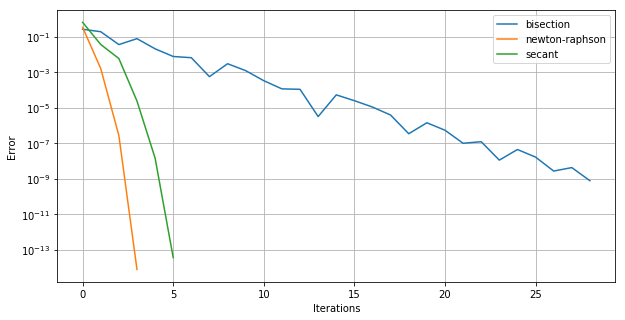
\includegraphics[width=.9\linewidth]{./obipy-resources/11275Nal.png}

Here we do see that the Newton-Raphson method slightly outperforms the secant
method, and both hugely outperform the bisection method.

\section*{Problem 3}
\label{sec-3}
We start with $e = .617139$, $T = 27906.98161$, $a = 2.34186 s \times
c$. We wish to solve for the elliptical orbit of the system by finding $\xi$ in
terms of $t$ and the equations for ${x, y}$ in terms of $\xi$.

We start by solving the equation $\frac{T}{2 \pi} (\xi - e \sin{\xi}) - t^* = 0$
and then plugging this value into the equations $x = a(\cos{\xi} - e), y = a
\sqrt{1 - e^2} \sin{\xi})$.

\begin{minted}[frame=lines,fontsize=\scriptsize]{python}
e_val = .617139
T_val = 27906.98161 # units of s
a_val = 2.34186 # units of s * c

def test_func(xi, tStar, e, T, a):
    return (T / (2 * np.pi)) * (xi - e * np.sin(xi)) - tStar

def xi_func(tStar, e, T, a):
    def xi_one_var(xi):
        return (T / (2 * np.pi)) * (xi - e * np.sin(xi)) - tStar
    return xi_one_var

def solve_xi(tStar, e, T, a):
    xi_solve_func = xi_func(tStar, e, T, a)
    secant_xi_solve = secant(xi_solve_func, 0, 2 * np.pi, tolerance_needed=.0001)
    return secant_xi_solve

def get_x_y(xi, e, a):
    x = a * (np.cos(xi) - e)
    y = a * np.sqrt(1 - e ** 2) * np.sin(xi)
    return (x, y)

def solve_pos(tStar, e, T, a):
    xi = solve_xi(tStar, e, T, a)
    x, y = get_x_y(xi, e, a)
    return (x, y)

def solve_orbit(e, T, a, tStar_vals):
    # solve for orbit in terms of other times
    xy_vals = list(map(lambda tStar: solve_pos(tStar, e, T, a), tStar_vals))
    return np.array(xy_vals)
\end{minted}


\begin{minted}[frame=lines,fontsize=\scriptsize]{python}
tStar_vals = np.linspace(-T_val / 2, T_val, 500)
orbit_solve = solve_orbit(e_val, T_val, a_val, tStar_vals)
x_vals = orbit_solve[::, 0]
y_vals = orbit_solve[::, 1]

plt.plot(x_vals, y_vals)
plt.xlabel('x-coordinate of orbit (s * c)')
plt.ylabel('y-coordinate of orbit (s * c)')
plt.grid()
plt.show()
\end{minted}

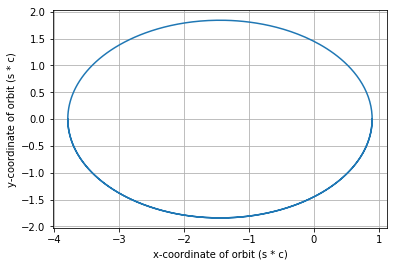
\includegraphics[width=.9\linewidth]{./obipy-resources/112750_r.png}

And here we see the orbit is an ellipse as expected!

\section*{Problem 4}
\label{sec-4}
We will obtain the velocities of the orbit through finite-difference formulas:
$$ x'(t) \approx [x(t + \Delta t) - x(t)] / \Delta t, y'(t) \approx [y(t +
\Delta t) - y(t)] / \Delta t$$

\begin{minted}[frame=lines,fontsize=\scriptsize]{python}
def get_velocity(pos_data, dt):
    # assume that dt is the same for each value in pos_data add array to index
    # + 1 (can cycically shift since last index and first index are connected
    # since orbit is periodic))
    velocity_data = (np.roll(pos_data, -1) - pos_data) / dt
    return velocity_data

def get_radial_vel(x_data, y_data, t_data, phi):
    dt = t_data[1] - t_data[0]
    x_vels = get_velocity(x_data, dt)
    y_vels = get_velocity(y_data, dt)
    # project {x'(t), y'(t)} onto unit vector (in terms of phi)
    r_vels = np.dot(np.array([x_vels, y_vels]).T, 
                    np.array([np.cos(phi), np.sin(phi)]))
    return r_vels
\end{minted}


After testing out various values of $\phi$, the value of $\frac{-\pi}{2}$ gave
the most qualitative agreement with Fig. 3 from the assignment:

\begin{minted}[frame=lines,fontsize=\scriptsize]{python}
r_vels = get_radial_vel(x_vals, y_vals, tStar_vals, -.5 * np.pi)
# Don't plot last value so that the last line doesn't go straight-up
# divide by the max to put in units of t/T
# convert to km / s
plt.plot((tStar_vals[:-1] / np.max(tStar_vals)), (r_vels * 3 * 10 ** 5)[:-1])
plt.xlabel('Phase (t / T)')
plt.ylabel('Radial Velocity (km / s)')
plt.grid()
plt.show()
\end{minted}

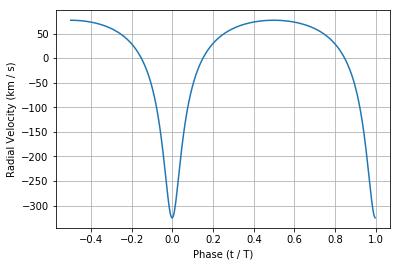
\includegraphics[width=.9\linewidth]{./obipy-resources/11275zTB.png}
% Emacs 25.2.1 (Org mode 8.2.10)
\end{document}
